\documentclass{article}

\usepackage[a4paper, total={6in, 8in}]{geometry}
\usepackage[utf8]{inputenc}
\usepackage{fancyhdr}
\usepackage{tabularx}
\usepackage{graphicx}
\usepackage{enumitem}
\usepackage{textcomp}
\usepackage{gensymb}

\pagestyle{fancy}
\fancyhf{}
\lhead{John J Li}
\rhead{CSE360 Summer 2021 Assignment 6}
\rfoot{\thepage}
\renewcommand{\headrulewidth}{0.4pt}

\setlength{\parskip}{1em}
\setlength\parindent{0px}
\title{CSE360 Summer 2021 Assignment 6}
\date{\today}
\author{John J Li}

\begin{document}
    \maketitle
    \thispagestyle{empty}
    \noindent\rule{\textwidth}{0.8pt}

    %################################################################################### 
    \section*{Problem 1}

    Create the flowchart, pseudocode, and Nassi-Shneiderman diagram that does the
    following:
    \begin{itemize}
        \item 
        Read in a number entered by the user
        \item
        If the number is 0 or a negative number, prompt the user to enter a different
        number
        \item
        Multiply the input number with every number between 1 and 20 and print the
        result of each multiplication
        \item
        Example, let’s say the user enters the number 5, the output would be: 5, 10, 15,
        20, …., 100
    \end{itemize}

    (a) Fill in the missing “???” parts of the below flowchart to have it model the
    algorithm described above.

    \begin{center}
        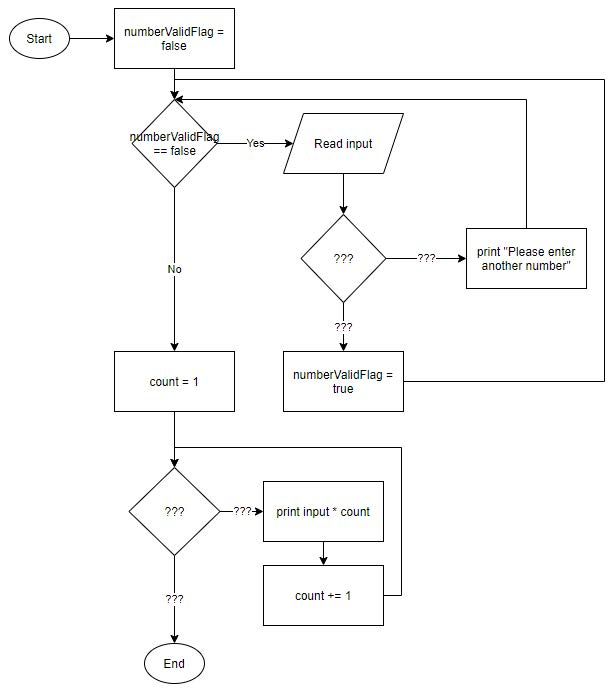
\includegraphics[scale=0.9]{Exercise 6_ Practice Problem 1.jpg}
    \end{center}

    \subsection*{Solution}

    \begin{center}
        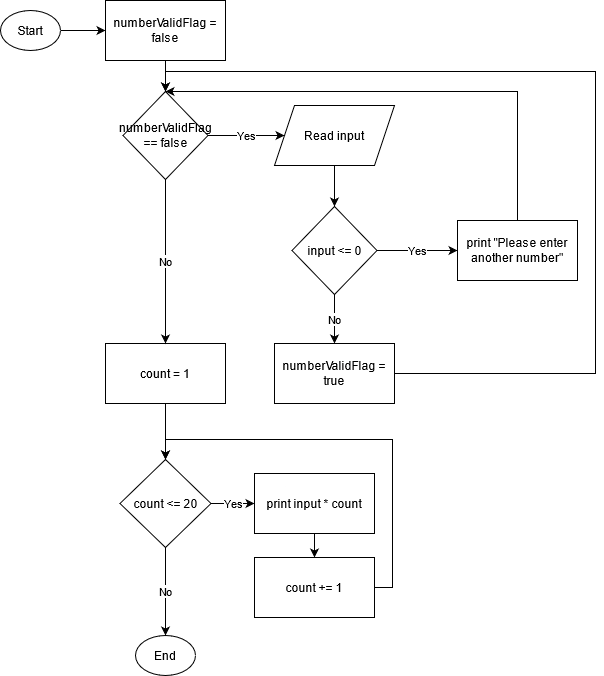
\includegraphics[scale=0.7]{Problem1_a.png}
    \end{center}

    (b) Fill in the missing “???” parts of the pseudo-code for the algorithm described
    above.

    \begin{verbatim}
    set numberValidFlag to false
    while( numberValidFlag == false )
        read input
        if( ??? )
            print “Please enter another number”
        else
            numberValidFlag = true
        end if
    end while

    set count to 1
    while ( ??? )
        print input * count
        count += 1
    end while
    \end{verbatim}

    \subsection*{Solution}
    
    \begin{verbatim}
    set numberValidFlag to false
    while( numberValidFlag == false )
        read input
        if(input <= 0)
            print “Please enter another number”
        else
            numberValidFlag = true
        end if
    end while

    set count to 1
    while (count <= 20)
        print input * count
        count += 1
    end while
    \end{verbatim}

    (c) Fill in the “???” part of the Nassi-Schneiderman diagram for this problem.

    \begin{center}
        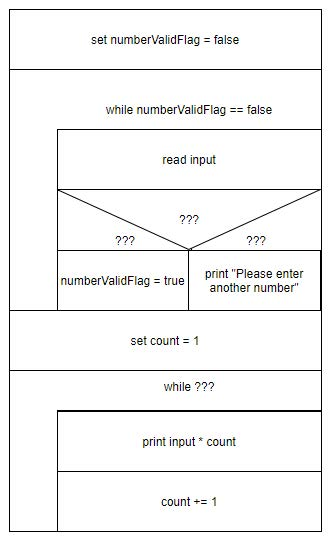
\includegraphics[scale=0.8]{Exercise 6_ Practice Problems c.jpg}
    \end{center}

    \subsection*{Solution}

    \begin{center}
        \includegraphics[scale=0.5]{problem1_c.png}
    \end{center}

    \section*{Problem 2}

    Write the algorithm for a program that calculates a moving average (also called a
    running average). The program will read 20 numbers from the user. As each number is
    read in, the average of the most recent 5 numbers will be calculated and the result is
    printed out.

    For example,

    \begin{verbatim}
    The first five input is 1, 2, 3, 4, 5   output: (1 + 2 + 3 + 4 + 5) / 5 = 3
    The next input is 6                     output: (2 + 3 + 4 + 5 + 6) / 5 = 4
    The next input is 7                     output: 5
    \end{verbatim}

    (a) Create a flowchart for the program.

    \subsection*{Solution}

    \begin{center}
        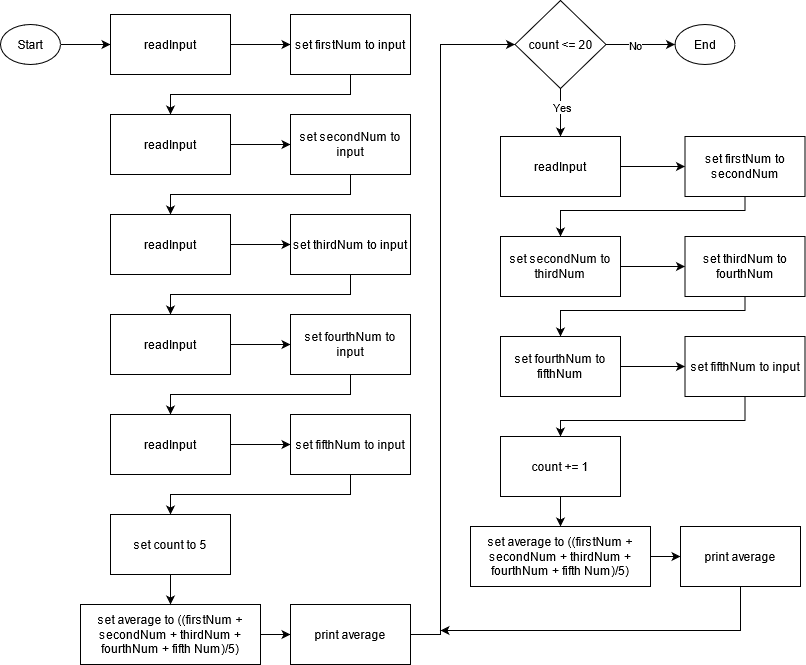
\includegraphics[scale=0.5]{Problem2_a.png}
    \end{center}

    (b) Write the pseudocode for the program.

    \subsection*{Solution}

    \begin{verbatim}

        read input 
        set firstNum to input
        read input
        set secondNum to input 
        read input 
        set thirdNum to input 
        read input 
        set fourthNum to input 
        read input 
        set fifthNum to input
        set count to 5

        set average to 
            ((firstNum + secondNum + thirdNum + fourthNum + fifthNum)/5)

        print average

        while ( count <= 20 )
            read input
            set firstNum to secondNum 
            set secondNum to thirdNum 
            set thirdNum to fourthNum 
            set fourthNum to fifthNum 
            set fifthNum to input
            count += 1

            set average to 
                ((firstNum + secondNum + thirdNum + fourthNum + fifthNum)/5)

            print average
        end while
    \end{verbatim}

    (c) Create a Nassi-Shneiderman diagram for the program.

    \subsection*{Solution}

    \begin{center}
        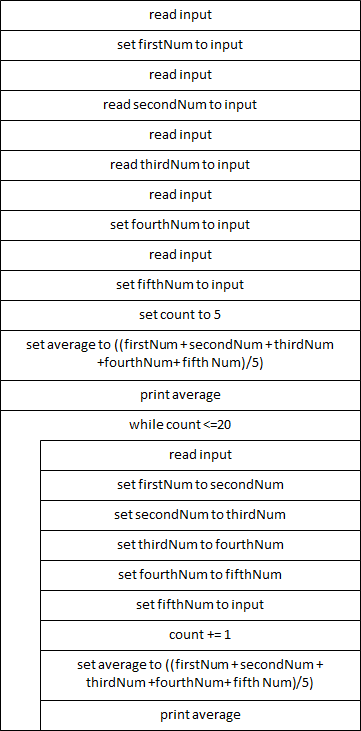
\includegraphics[scale=0.6]{Problem2_c.png}
    \end{center}

\end{document}